\section{Versuchsaufbau und Durchführung}
\label{sec:experimental_setup_and_conduction}
\subsection{Versuchsaufbau}
\label{sec:versuchsaufbau}
\begin{figure}[h]
\centering
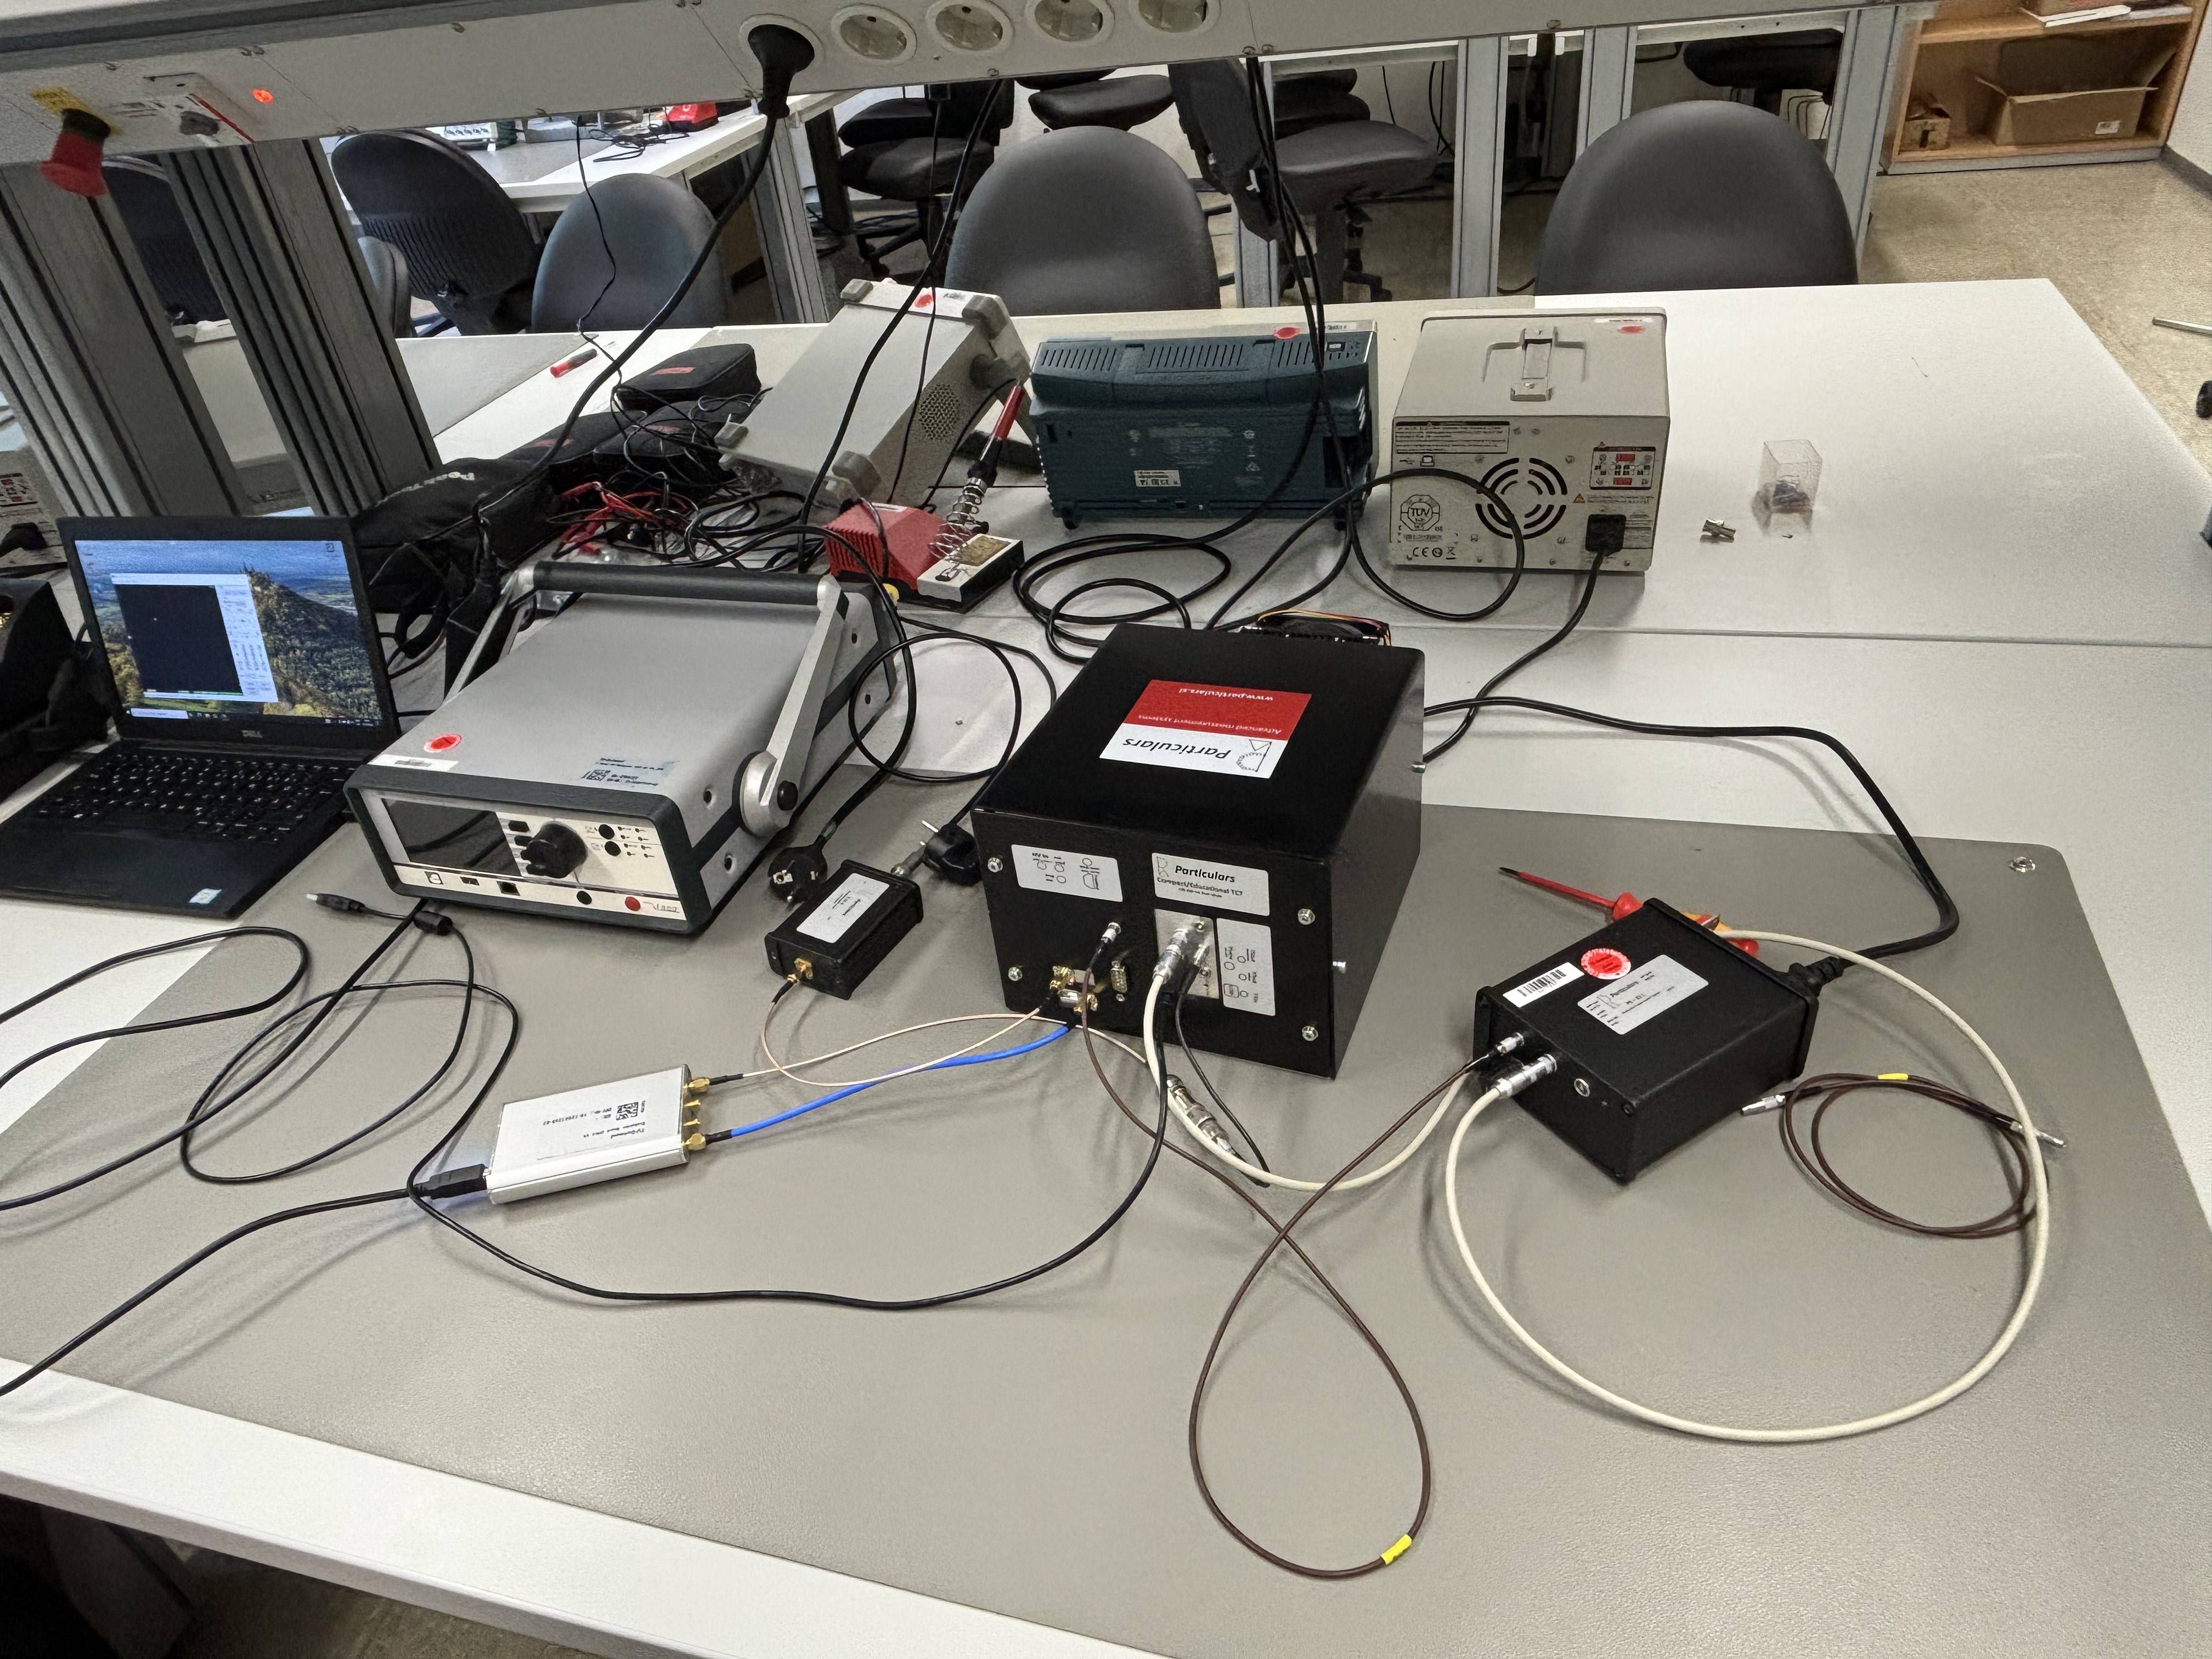
\includegraphics[width=\textwidth]{content/Figures/setup.png}
\caption{Der Versuchsaufbau der Messung des Drifts von Ladungsträgern mit der Transient-Current-Technik (TCT).}
\label{fig:setup}
\end{figure}
\begin{figure}[h]
\centering
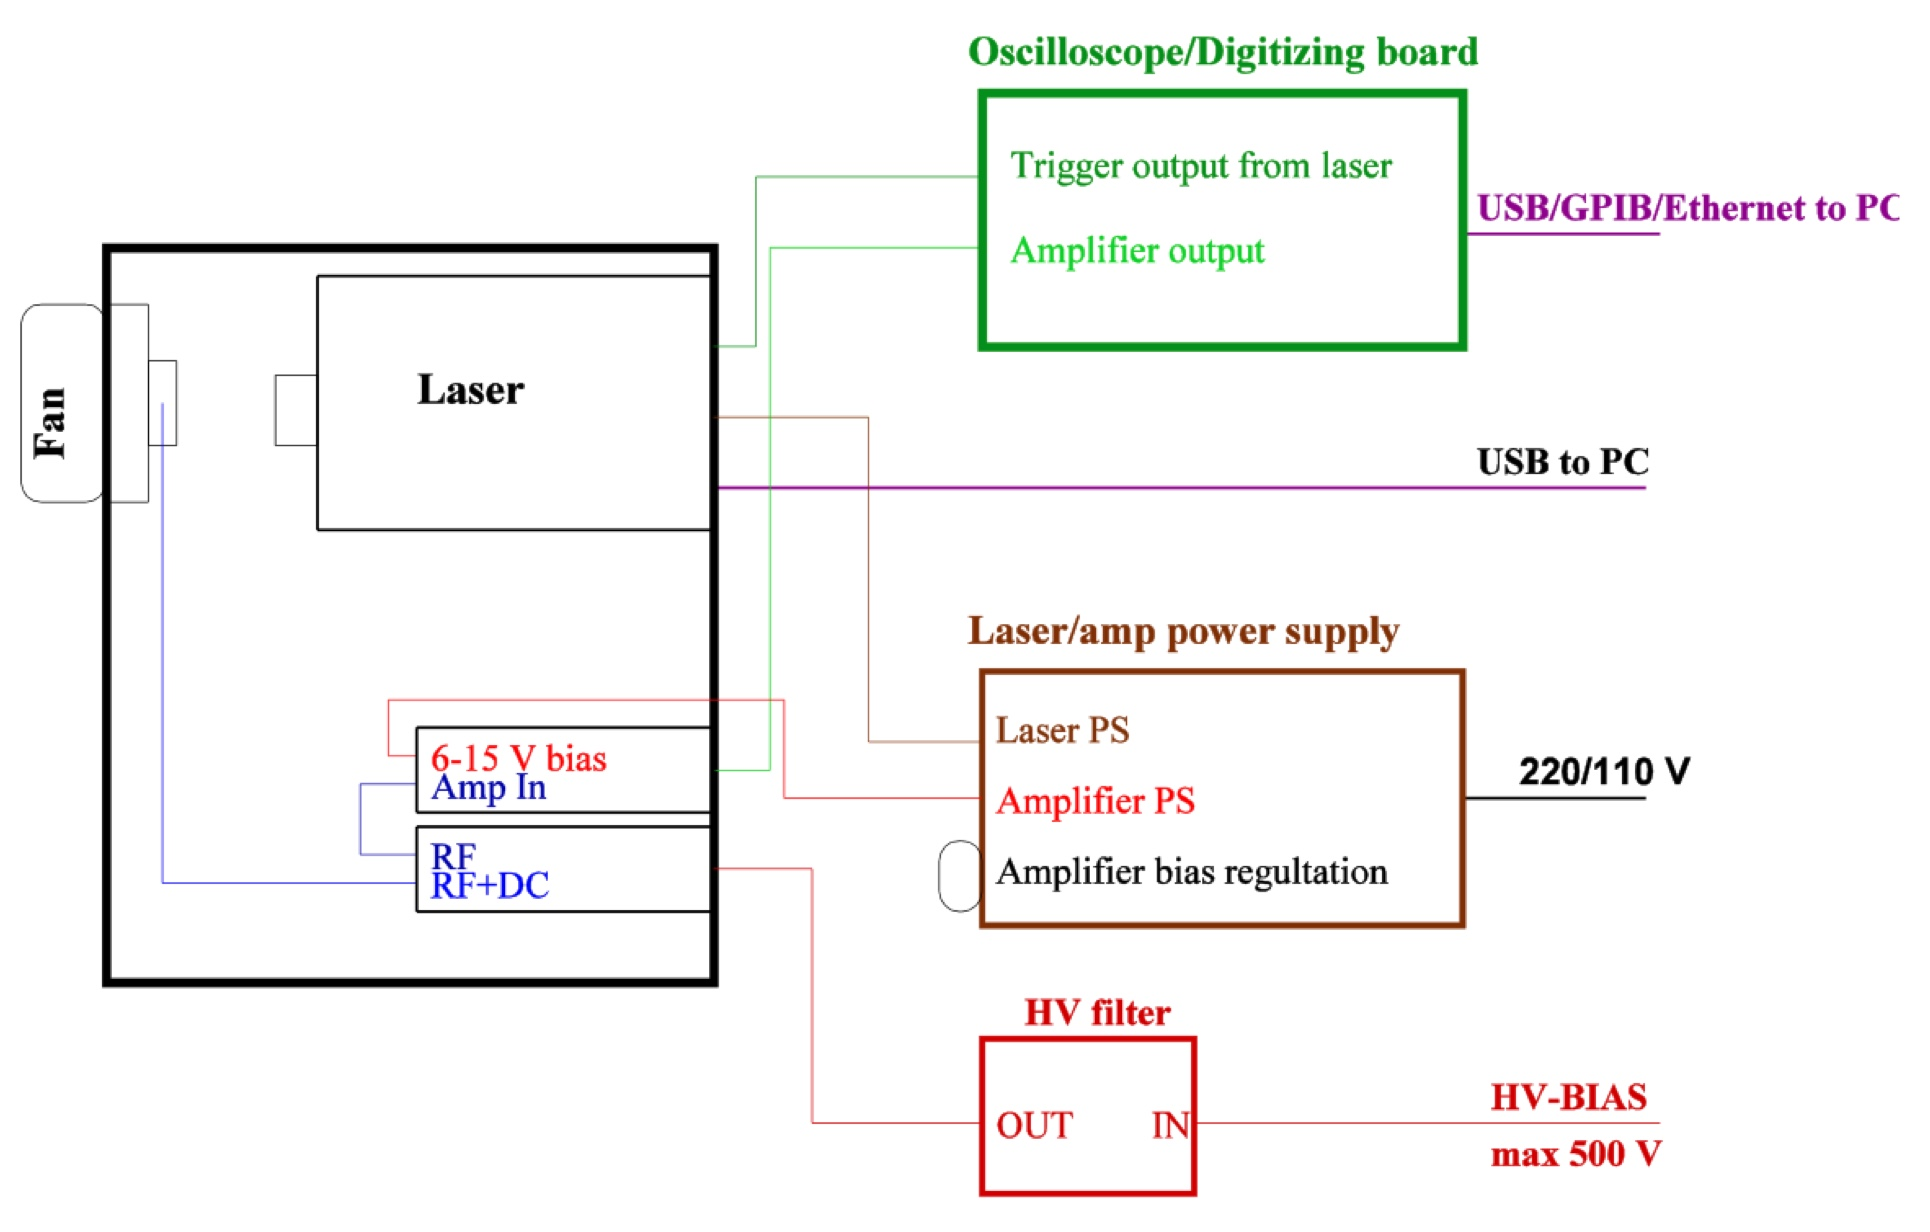
\includegraphics[width=\textwidth]{content/Figures/schem_setup.jpg}
\caption{Schematischer Aufbau des Experiments \cite{Anleitung}.}
\label{fig:schem_setup}
\end{figure}
\subsection{Versuchsdurchführung}
\label{sec:versuchsdurchführung}